\chapter{Analiza technologiczna i narzędzia}
\section{Narzędzia i biblioteki}
\subsection{Google Colaboratory}

\hspace{0.5cm}
Google Colaboratory lub Colab jest to usługa w chmurze od Google Research. IDE opierające się na środowisku Jupyter Notebook, przeznaczone jest do szkoleń i badań w zakresie uczenia maszynowego. Google Colab udostępnia darmowy dostęp do układów GPU, TPU i~dużych zasobów pamięci, które umożliwiają i przyspieszają proces uczenia sieci.

Utworzona maszyna wirtualna jest dostępna dla użytkownika tylko na ograniczony czas ciągłej pracy (ok. 12 godzin) i jest przeznaczona do interaktywnego korzystania z notatnika. Oznacza to, że zostanie ona usunięta, a zasoby pamięci zwolnione po określonym czasie działania programu, braku aktywności ze strony użytkownika lub przekroczeniu dostępnej pamięci. 


\subsection{Python}
\hspace{0.5cm}
Python jest wysokopoziomowym językiem programowania obiektowego ogólnego przeznaczenia, szczególnie popularnym w dziedzinach związanych z data science lub uczeniem maszynowym. Razem z Pythonem w wersji 3.9 zainstalowane zostały m.in biblioteka numpy, pillow czy kompiler cython.

\subsection{Tensroflow, Tensorboard i Keras}

\hspace{0.5cm}
Tensorflow to stworzona przez Google Brain Team biblioteka przeznaczona do realizacji projektów z dziedziny uczenia maszynowego oraz głębokich sieci neuronowych. Architektura biblioteki umożliwia wykonywanie obliczeń z wykorzystaniem jednej lub większej liczby procesorów lub kart graficznych bez konieczności wymiany uruchamianego kodu.

Tensorflow oferuje również zbiór narzędzi służących do wizualizacji danych, TensorBoard. Pozwala on prezentować m.in. grafy obliczeniowe sieci neuronowych, postęp treningu i walidacji sieci ułatwiając tym samym ewaluację oraz optymalizację ich działania.

Pakiet Keras, jest to otwarto-źródłowa biblioteka, umożliwiająca uruchamianie, tworzenie i~trenowanie dowolnych modeli sieci neuronowych. Implementacja pakietu Keras jest uniezależniona od jednej biblioteki obsługującej tensory tj. TensorFlow, Theano lub Microsoft Cognitive Toolkit, jednak standardowo wykorzystywana jest jako API współdziałające z TensorFlow.


\subsection{OpenCv}
\hspace{0.5cm}OpenCV jest bezpłatną i opensource'ową biblioteką funkcji służących do zaawansowanego przetwarzania i obróbki obrazu w czasie rzeczywistym. Biblioteka oferuje obszerny zestaw algorytmów służących m.in. do rozpoznawania i~identyfikowania twarzy oraz obiektów, klasyfikowania działań ludzkich na materiale filmowym\cite{OpenCV}, funkcji wizualizujących przetwarzane obrazy i wielu innych działań wykorzystywanych w aplikacjach wizyjnych i uczeniu maszynowym.

\section{Architektura sieci}
\hspace{0.5cm}
Jako model wykrywania obiektów zastosowany został RetinaNet, zaproponowany przez zespół badawczy Facebook AI. Jest to jeden z najpopularniejszych jednoetapowych modeli wykrywania obiektów (ang. \emph{one-stage object detection model}) specjalizujący się w rozpoznawaniu elementów o małej skali. Jednoetapowe detektory wymagają jedynie jednego przejścia danych przez sieć neuronową w celu przewidzenia wszystkich pól występowania obiektów. Takie szybkie rozwiązanie jest często pożądane w aplikacjach mobilnych. Innymi detektorami jednoetapowymi są np. sieci YOLO, SqueezeNet lub DetectNet.

Cała struktura RetinaNet składa się z sieci szkieletowej (ang. \emph{backbone}) i dwóch podsieci zadaniowych odpowiadających za klasyfikację i wyprowadzenie regresji. Szkielet modelu jest samodzielną siecią konwolucyjną, która jest odpowiedzialna za obliczenie splotowej mapy cech nad całym obrazem wejściowym. Kolejne dwie podsieci odpowiedzialne są odpowiednio za splotową klasyfikację obiektów będących danymi wyjściowymi sieci szkieletowej oraz splotową regresję ramki ograniczającej.


\begin{figure}[H]
    \centering
    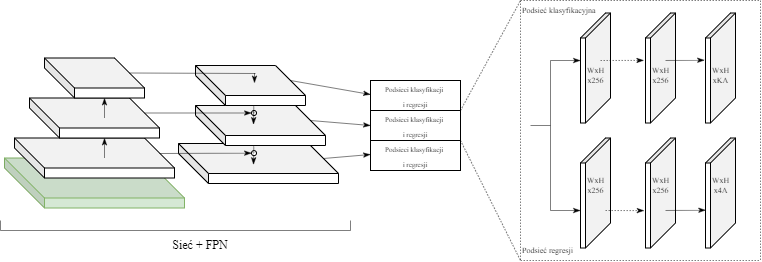
\includegraphics[width=0.9\linewidth]{Obrazy/Rozdzial04/retinanet.png}
    \caption{Architektura podejścia RetinaNet.}
    \label{fig:retinanet}
\end{figure}

Model RetinaNet zazwyczaj występuje w parze z architekturą Resnet, możliwe są inne implementacje. Biblioteka Keras oraz repozytorium \cite{Fizyr}, które zostało wykorzystane do trenowania sieci implementują różne warianty sieci ResNet w zależności od ilości warstw. Do badań zostały wybrane trzy rodzaje: 50, 101 i 152 warstwowe oraz VGG19.

\subsection{ResNet}
\hspace{0.5cm}
Sieci typu ResNet to struktury sieciowe zaproponowane w 2015 roku przez członków Microsoft Research Asia - Kaiming He, Xiangyu Zhang, Shaoqing Ren and Jian Sun. \cite{ResNet}. Ideą stojącą za powstaniem tej struktury były problemy znikającego gradientu występujące w przypadku coraz głębszych sieci. Zwiększanie liczby stosowanych warstw jest często kluczowym elementem usprawniania działania tworzonych modeli, jednak w przypadku przekroczenia pewnej granicznej liczby warstw w sieciach konwolucyjnych, powodowało ono jednoczesne zwiększenie się błędu w trakcie uczenia zarówno na zbiorze walidacyjnym, jak i trenującym. Wyciągniętym wnioskiem było stwierdzenie, że zbyt głębokie sieci neuronowe są ciężkie do zoptymalizowania  \cite{ResNet}.

Główną częścią sieci ResNet jest przedstawiony na rysunku \ref{fig:resnet} moduł rezydualny

\begin{figure}[H]
    \centering
    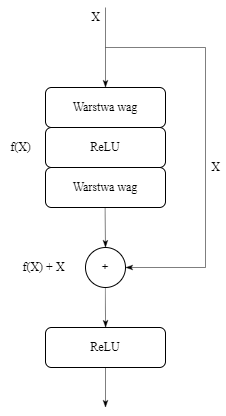
\includegraphics[width=0.3\linewidth]{Obrazy/Rozdzial04/modelrezydualny.png}
    \caption{Moduł z połączeniem rezydualnym ResNet.}
    \label{fig:resnet}
\end{figure}

Podczas treningu sieci, nie uczy się ona pewnego przekształcenia $h(\textbf{X})$, ale poznaje przybliżenie funkcji rezydualnej $F(\textbf{X}) = h(\textbf{X}) - \textbf{X}$, gdzie $\textbf{X}$ jest pewną wartością wejściową. 

Wartość rezydualna sieci powinna być uczona w taki sposób, aby zbliżała się do zera, tak aby blok resztkowy reprezentował optymalne przekształcenie tożsamościowe. W ten sposób wszystkie warstwy w sieci zawsze będą tworzyć optymalne mapy cech, tj. najlepszą mapę cech po operacjach splotu, łączenia i aktywacji \cite{Resnet2}.

\subsection{VGG}

\hspace{0.5cm}
Architektura VGGNet została przedstawiona przez Visual Geometry Group, jako część badań poświęconych modelom sieci o rosnącej głębokości przy zastosowaniu filtrów konwolucyjnych o małych wymiarach. Jest to klasyczna sieć konwolucyjna stosowana do klasyfikacji obrazów. Wyróżnia się kilka architektur od 11 do 19 warstw, gdzie do najpopularniejszych należą VGG16 oraz VGG19. W każdej z możliwych wersji wykorzystywane są małe filtry $3x3$ lub $1x1$, zgodnie z zaleceniami autorów VGG \cite{ResNet}.


% Z kolei główną zaletą sieci binarnych jest niewielki rozmiar wyuczonego modelu, co umożliwia jego zastosowanie w urządzeniach o niewielkiej mocy obliczeniowej. Wynika to z faktu, że wagi połączeń pomiędzy neuronami występują jedynie w postaci binarnej.
\section{Zbiór danych}

\hspace{0.5cm}
Jako dane do nauki sieci wykorzystane zostały dwa zestawy danych. Aby móc je wykorzystać w uczeniu i zadaniu wykrywania obiektów na obrazie adnotacje, kategorie i ścieżki do plików obu zbiorów zostały zamienione na format COCO \cite{CistyscapesToCOCO}. Format ten jest specyficznym rodzajem struktury plików JSON, dyktującym sposób zapisywania etykiet (adnotacji) i metadanych dla różnych zestawów danych obrazów.

\begin{figure}[H]
    \centering
    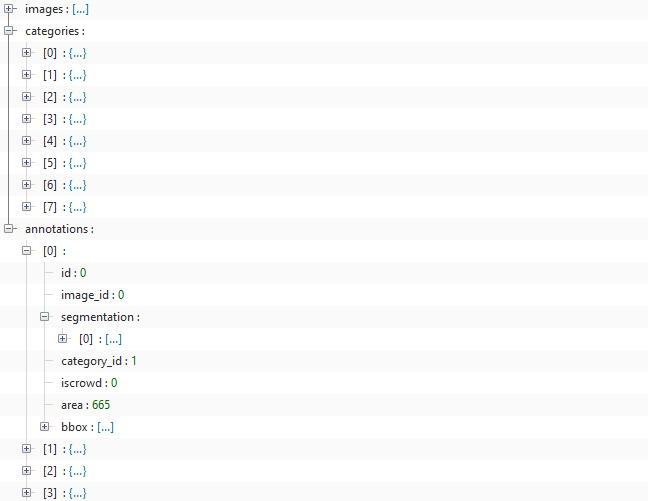
\includegraphics[width=0.7\linewidth]{Obrazy/Rozdzial04/coco.png}
    \caption{Struktura odpowiednio przygotowanego zbioru danych w formacie COCO.}
    \label{fig:coco}
\end{figure}

\hspace{0.5cm}
W tak przygotowanym pliku można wyróżnić trzy kategorie
\begin{itemize}
    \item[--] images - lista wszystkich dostępnych zdjęć i podstawowych informacji o nich,
    \item[--] categories - określa jakie obiekty na obrazie model jest w stanie wykryć i opisać,
    \item[--] annotations - lista wszystkich adnotacji poszczególnych obiektów z każdego obrazu należącego do zbioru danych.
\end{itemize}

\subsection{CityScapes Dataset}

\hspace{0.5cm}
CityScapes Dataset \cite{Cordts2016Cityscapes} to ogólnodostępna baza danych, skoncentrowana na przedstawieniu sytuacji ulicznych. Dane zebrano w 50 miastach w ciągu kilku miesięcy, w ciągu dnia i~przy dobrych warunkach pogodowych. Pierwotnie została stworzona jako wideo, następnie klatki zostały ręcznie wybrane tak, aby miały następujące cechy: duża liczba obiektów dynamicznych, zmienny układ scen i zmienne tło \cite{CityscapesPapers}. Do dyspozycji użytkownika przeznaczone zostało 8 różnych klas, służących do oznaczenia ludzi i pojazdów
\begin{itemize}
    \item[--] pieszy (ang. \emph{person}),
    \item[--] jeździec (ang. \emph{rider}),
    \item[--] samochód (ang. \emph{car}),
    \item[--] rower (ang. \emph{bicycle}),
    \item[--] motocykl (ang. \emph{motorcycle}),
    \item[--] autobus (ang. \emph{bus}),
    \item[--] ciężarówka (ang. \emph{truck}),
    \item[--] pociąg (ang. \emph{train}).
\end{itemize}


\begin{figure}[H]
    \centering
    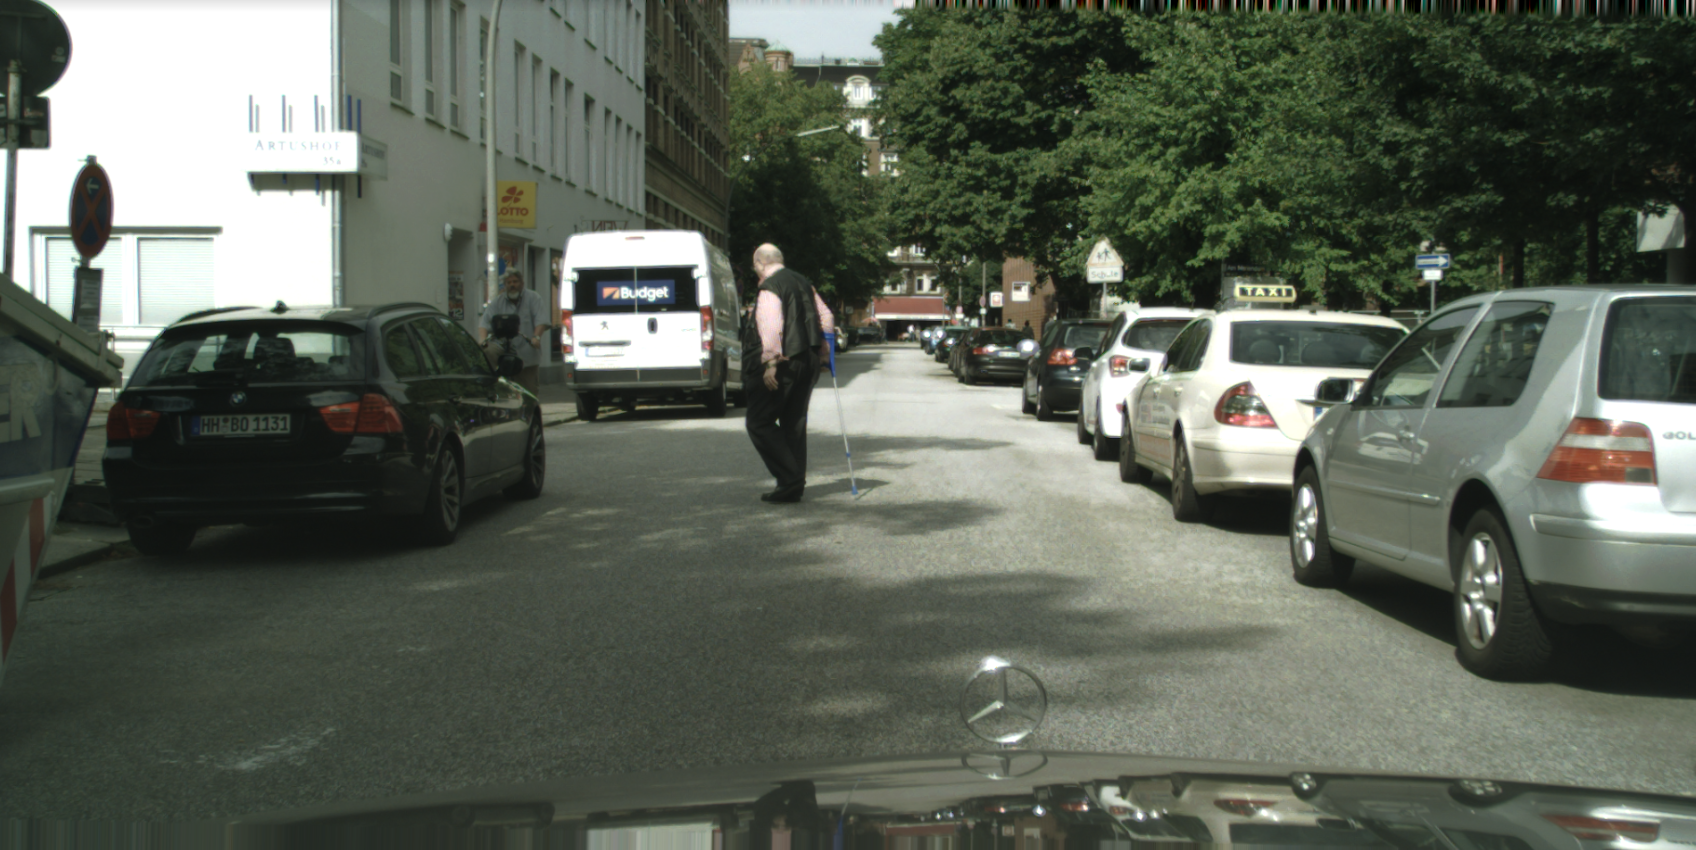
\includegraphics[width=0.9\linewidth]{Obrazy/Rozdzial04/cityscapes.png}
    \caption{Zdjęcie z zestawu danych Cityscapes.}
    \label{fig:cityscapes}
\end{figure}


\hspace{0.5cm}
W celu przyspieszenia procesu nauki sieci cały zbiór danych został zmniejszony do 1200 zdjęć wykorzystanych do treningu i około 300 zdjęć wybranych do ewaluacji modelu.

\subsection{Mendeley Data RDD2020}

\hspace{0.5cm}
Zbiór RDD2020\cite{MendeleyData} zawiera ponad 26 tysięcy zdjęć przedstawiających uszkodzenia w nawierzchni drogi oraz prostokątne adnotacje. Wszystkie zdjęcia wykonane zostały za pomocą telefonów komórkowych zamontowanych w pojazdach. Obszerny zbiór łączący w sobie dane z~Japonii, Indii i Czech rozróżnia różne rodzaje zniszczonej nawierzchni m.in. pęknięcia występujące wzdłuż drogi, pęknięcia poprzeczne, studzienki.

\begin{figure}[H]
    \centering
    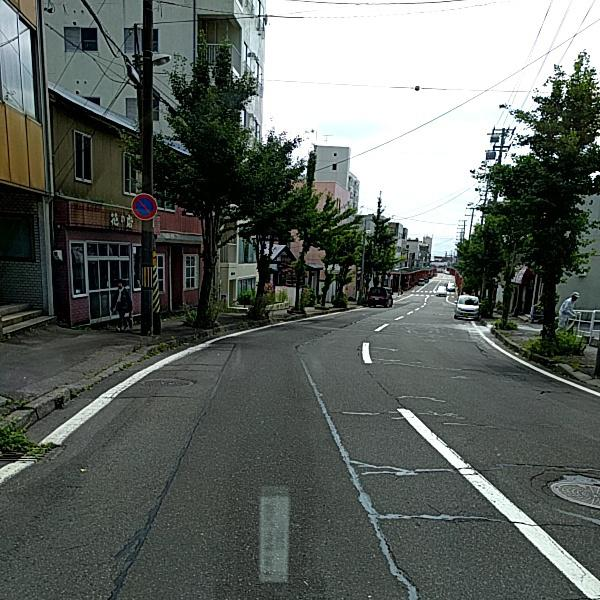
\includegraphics[width=0.5\linewidth]{Obrazy/Rozdzial04/mendeley.jpg}
    \caption{Zdjęcie z zestawu danych RDD2020.}
    \label{fig:mendeley}
\end{figure}


% \begin{multicols}{2}
% \begin{itemize}
%     \item[--] D00 - pęknięcia wzdłuż drogi,
%     \item[--] D01
%     \item[--] D10 - pęknięcia poprzeczne,
%     \item[--] D11
%     \item[--] D20 - pęknięcia przypominające skórę aligatora,
%     \item[--] D30
%     \item[--] D40 - studzienki.
%     \item[--] D43
%     \item[--] D44
%     \item[--] D50
% \end{itemize}
% \end{multicols}


\hspace{0.5cm}
Podobnie jak w przypadku zbioru CityScapes, dane pochodzące z Mendeley Data również zostały zmniejszone do ok. 1000 plików treningowych i 300 plików walidacyjnych.

\subsection{Filmy wykonane samodzielnie}
\label{r:sanok}
\hspace{0.5cm}
Dodatkowo za pomocą kamery samochodowej zostało wykonanych kilka krótkich nagrań ruchu drogowego.

% \begin{figure}[H]
%     \centering
%     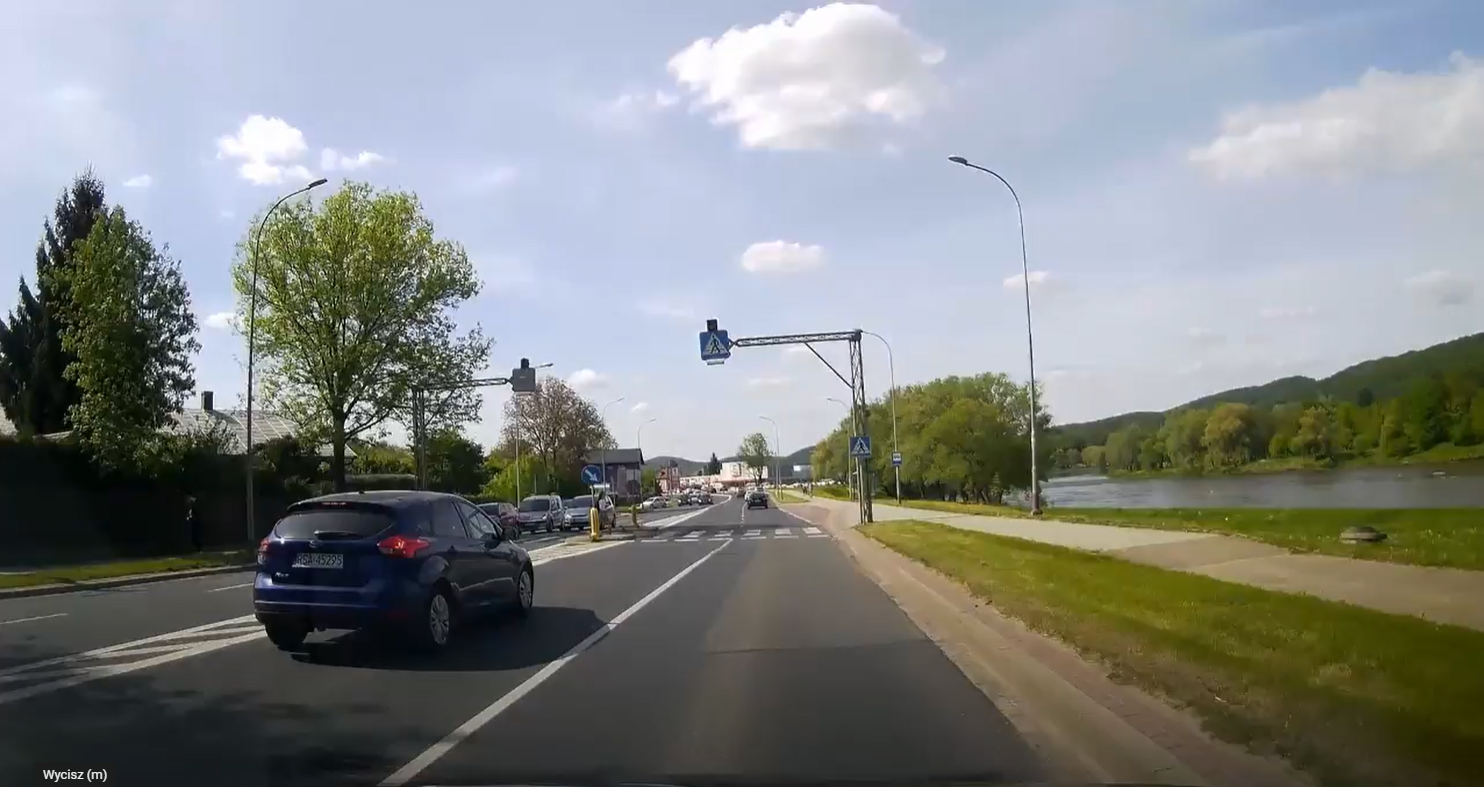
\includegraphics[width=0.8\linewidth]{Obrazy/Rozdzial04/wlasne.png}
%     \caption{Przykładowa klatka filmu z kamery samochodowej.}
%     \label{fig:sanok}
% \end{figure}

\begin{figure}[H]
\centering
        \subfloat[Przykładowa klatka filmu z kamery samochodowej.]{\label{wlasn1}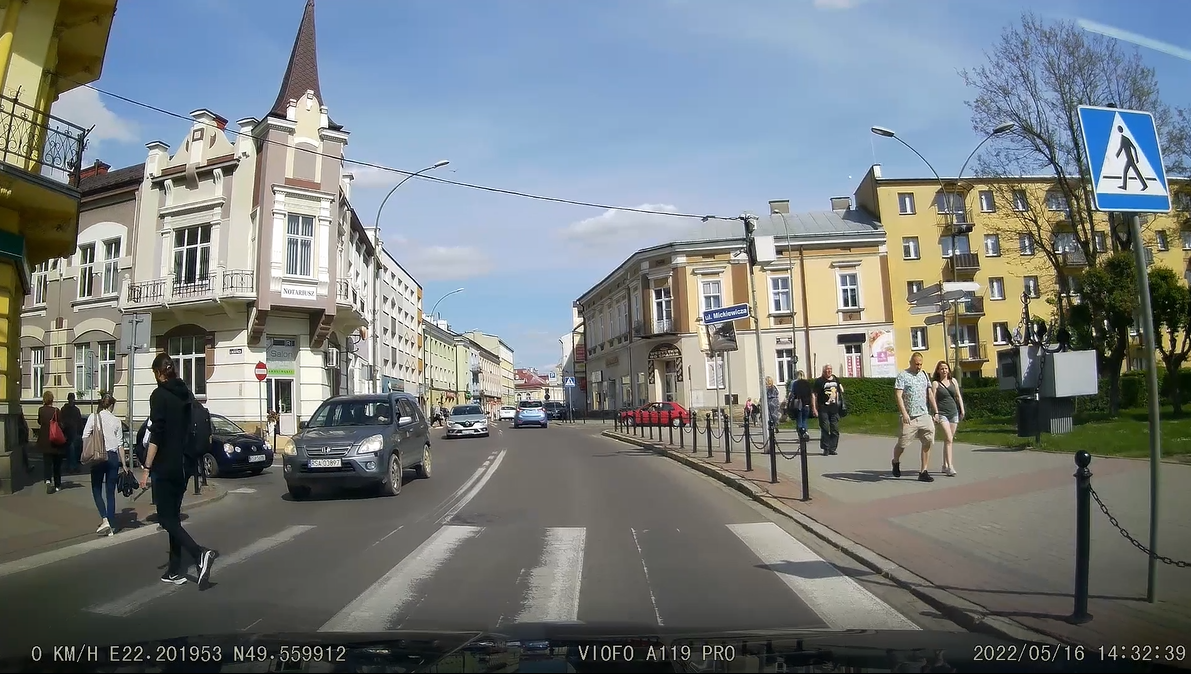
\includegraphics[width=.7\linewidth]{Obrazy/Rozdzial04/w1}}\hfill
        \subfloat[Przykładowa klatka filmu z kamery samochodowej.]{\label{wlasn2}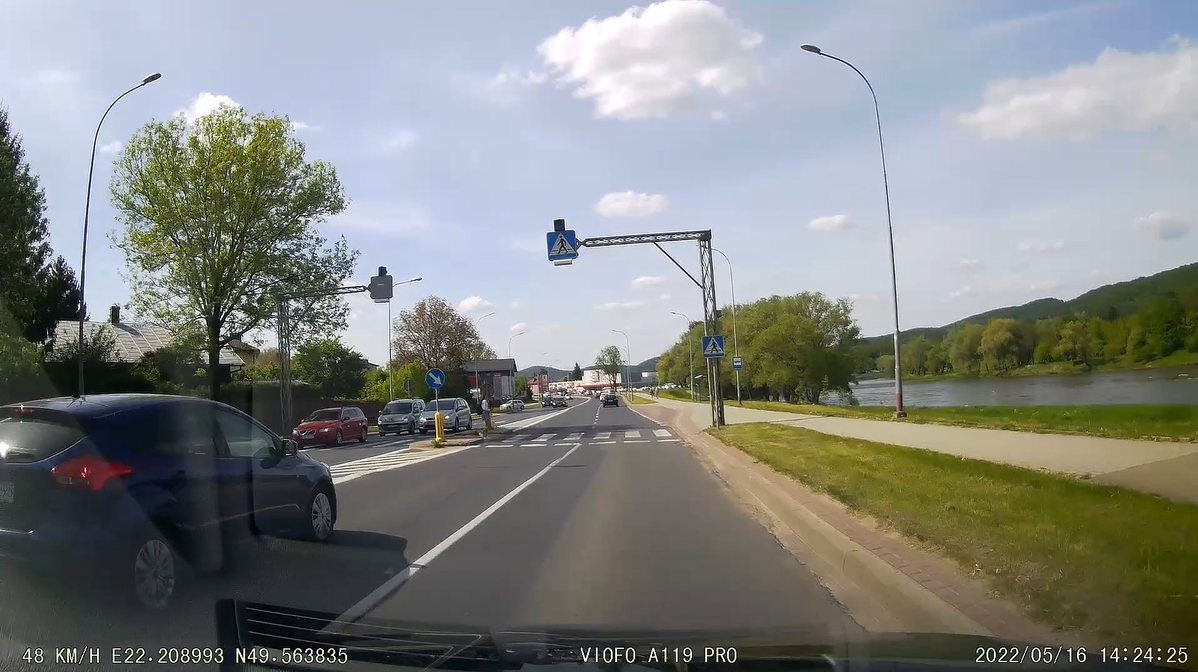
\includegraphics[width=.7\linewidth]{Obrazy/Rozdzial04/w4}}\hfill
        \subfloat[Przykładowa klatka filmu z kamery samochodowej.]{\label{wlasn3}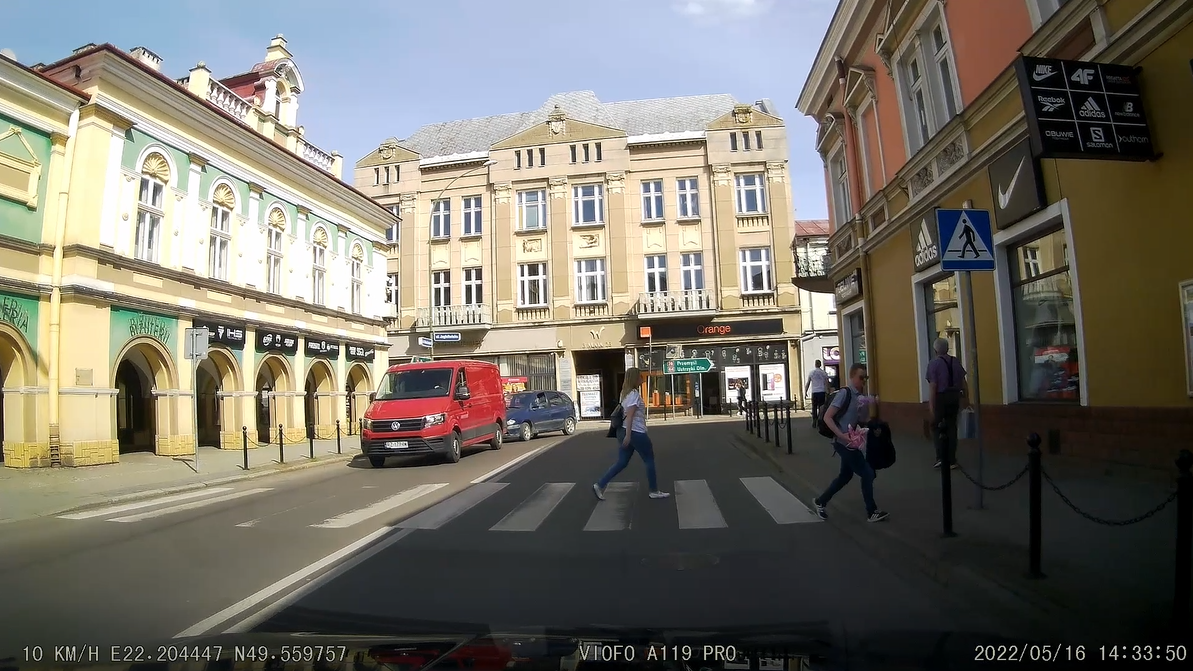
\includegraphics[width=.7\linewidth]{Obrazy/Rozdzial04/w2}}\hfill
    \caption{Fragmenty różnych filmów wykonanych na drodze.}
    \label{fig:sanok}
\end{figure}

